\subsection{State feedback design}
\label{statfeedback_d}

The open loop poles of the system are calculated as follows: 

\begin{equation}
  \label{eq:feedbackd}
    det(z\mathbf{I}-\mathbf{A}_d)
  \end{equation}

The open loop poles of the system as can be seen in \eqref{eq:openlooppoles_d} are in the unit circle which means, the system is stable: 

\begin{equation}
  \label{eq:openlooppoles_d}
  p_{{1;2}} = 0.8977 \pm j0.2585
  \end{equation}

The desired poles should be further to the origin of the z-plane, however should be also chosen carefully. Fast dynamics mean bigger state feedback gain, which can result in unwanted overshoots because of the outer control loop. For immediate changes in the disturbance, the system might react faster, however when the feedback gain is high, that would result in high overshoots. Considering that, the desired poles are first set to: 

\begin{equation}
  \label{eq:openlooppoles_d}
  p_{F_{1;2}} = 0.7 \pm j0.2585
  \end{equation} 
  
The state feedback gain yields: 
  
  \begin{equation}
\label{eq:F_d}
    F
=
 \begin{bmatrix}
    -9.61 & -53.51
\end{bmatrix}
\end{equation}
  
  With this state feedback, the following dynamics can be achieved:
  
\begin{figure}[H]
\centering
% This file was created by matlab2tikz.
%
%The latest updates can be retrieved from
%  http://www.mathworks.com/matlabcentral/fileexchange/22022-matlab2tikz-matlab2tikz
%where you can also make suggestions and rate matlab2tikz.
%
\definecolor{mycolor1}{rgb}{0.00000,0.44700,0.74100}%
\definecolor{mycolor2}{rgb}{0.85000,0.32500,0.09800}%
%
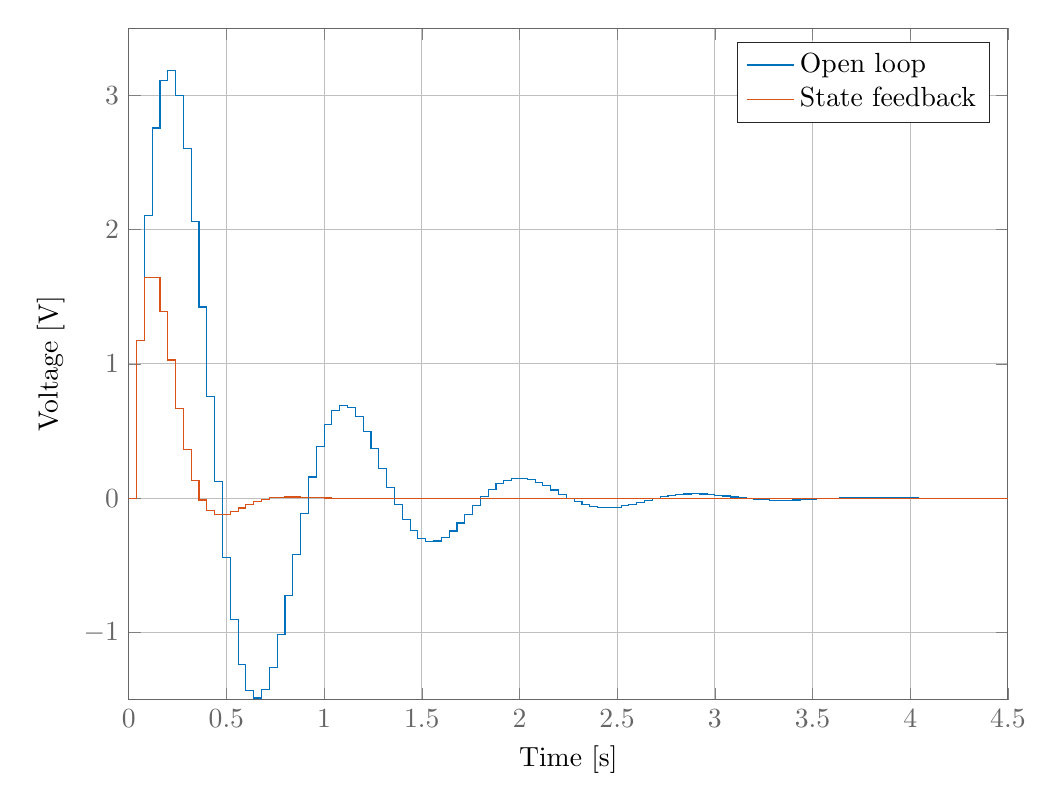
\begin{tikzpicture}

\begin{axis}[%
width=4.396in,
height=3.357in,
at={(0.883in,0.481in)},
scale only axis,
separate axis lines,
every outer x axis line/.append style={white!40!black},
every x tick label/.append style={font=\color{white!40!black}},
xmin=0,
xmax=4.5,
xlabel={Time [s]},
xmajorgrids,
every outer y axis line/.append style={white!40!black},
every y tick label/.append style={font=\color{white!40!black}},
ymin=-1.5,
ymax=3.5,
ylabel={Voltage [V]},
ymajorgrids,
axis background/.style={fill=white},
legend style={legend cell align=left,align=left,draw=white!15!black}
]
\addplot [color=mycolor1,solid]
  table[row sep=crcr]{%
0	0\\
0.04	0\\
0.04	1.173\\
0.08	1.173\\
0.08	2.106\\
0.12	2.106\\
0.12	2.757\\
0.16	2.757\\
0.16	3.112\\
0.2	3.112\\
0.2	3.182\\
0.24	3.182\\
0.24	2.996\\
0.28	2.996\\
0.28	2.603\\
0.32	2.603\\
0.32	2.058\\
0.36	2.058\\
0.36	1.424\\
0.4	1.424\\
0.4	0.7597\\
0.44	0.7597\\
0.44	0.1216\\
0.48	0.1216\\
0.48	-0.4446\\
0.52	-0.4446\\
0.52	-0.9045\\
0.56	-0.9045\\
0.56	-1.236\\
0.6	-1.236\\
0.6	-1.43\\
0.64	-1.43\\
0.64	-1.488\\
0.68	-1.488\\
0.68	-1.424\\
0.72	-1.424\\
0.72	-1.258\\
0.76	-1.258\\
0.76	-1.016\\
0.8	-1.016\\
0.8	-0.726\\
0.84	-0.726\\
0.84	-0.4169\\
0.88	-0.4169\\
0.88	-0.1149\\
0.92	-0.1149\\
0.92	0.1576\\
0.96	0.1576\\
0.96	0.3832\\
1	0.3832\\
1	0.5504\\
1.04	0.5504\\
1.04	0.6538\\
1.08	0.6538\\
1.08	0.6935\\
1.12	0.6935\\
1.12	0.6746\\
1.16	0.6746\\
1.16	0.6058\\
1.2	0.6058\\
1.2	0.499\\
1.24	0.499\\
1.24	0.3672\\
1.28	0.3672\\
1.28	0.2238\\
1.32	0.2238\\
1.32	0.08129\\
1.36	0.08129\\
1.36	-0.04934\\
1.4	-0.04934\\
1.4	-0.1595\\
1.44	-0.1595\\
1.44	-0.2434\\
1.48	-0.2434\\
1.48	-0.2977\\
1.52	-0.2977\\
1.52	-0.3221\\
1.56	-0.3221\\
1.56	-0.3185\\
1.6	-0.3185\\
1.6	-0.2907\\
1.64	-0.2907\\
1.64	-0.244\\
1.68	-0.244\\
1.68	-0.1844\\
1.72	-0.1844\\
1.72	-0.1181\\
1.76	-0.1181\\
1.76	-0.05108\\
1.8	-0.05108\\
1.8	0.01135\\
1.84	0.01135\\
1.84	0.06495\\
1.88	0.06495\\
1.88	0.1067\\
1.92	0.1067\\
1.92	0.1349\\
1.96	0.1349\\
1.96	0.1491\\
2	0.1491\\
2	0.1499\\
2.04	0.1499\\
2.04	0.1391\\
2.08	0.1391\\
2.08	0.1188\\
2.12	0.1188\\
2.12	0.092\\
2.16	0.092\\
2.16	0.06146\\
2.2	0.06146\\
2.2	0.03005\\
2.24	0.03005\\
2.24	0.0003209\\
2.28	0.0003209\\
2.28	-0.02565\\
2.32	-0.02565\\
2.32	-0.04634\\
2.36	-0.04634\\
2.36	-0.0608\\
2.4	-0.0608\\
2.4	-0.06873\\
2.44	-0.06873\\
2.44	-0.07033\\
2.48	-0.07033\\
2.48	-0.06629\\
2.52	-0.06629\\
2.52	-0.05764\\
2.56	-0.05764\\
2.56	-0.04564\\
2.6	-0.04564\\
2.6	-0.03163\\
2.64	-0.03163\\
2.64	-0.01696\\
2.68	-0.01696\\
2.68	-0.002842\\
2.72	-0.002842\\
2.72	0.009696\\
2.76	0.009696\\
2.76	0.01989\\
2.8	0.01989\\
2.8	0.02725\\
2.84	0.02725\\
2.84	0.03156\\
2.88	0.03156\\
2.88	0.03289\\
2.92	0.03289\\
2.92	0.0315\\
2.96	0.0315\\
2.96	0.02785\\
3	0.02785\\
3	0.02252\\
3.04	0.02252\\
3.04	0.01612\\
3.08	0.01612\\
3.08	0.009292\\
3.12	0.009292\\
3.12	0.002612\\
3.16	0.002612\\
3.16	-0.003419\\
3.2	-0.003419\\
3.2	-0.008418\\
3.24	-0.008418\\
3.24	-0.01213\\
3.28	-0.01213\\
3.28	-0.01443\\
3.32	-0.01443\\
3.32	-0.01533\\
3.36	-0.01533\\
3.36	-0.01492\\
3.4	-0.01492\\
3.4	-0.01341\\
3.44	-0.01341\\
3.44	-0.01106\\
3.48	-0.01106\\
3.48	-0.008151\\
3.52	-0.008151\\
3.52	-0.004982\\
3.56	-0.004982\\
3.56	-0.001831\\
3.6	-0.001831\\
3.6	0.00106\\
3.64	0.00106\\
3.64	0.003501\\
3.68	0.003501\\
3.68	0.005361\\
3.72	0.005361\\
3.72	0.00657\\
3.76	0.00657\\
3.76	0.007117\\
3.8	0.007117\\
3.8	0.007044\\
3.84	0.007044\\
3.84	0.006435\\
3.88	0.006435\\
3.88	0.005407\\
3.92	0.005407\\
3.92	0.004091\\
3.96	0.004091\\
3.96	0.002627\\
4	0.002627\\
4	0.001145\\
4.04	0.001145\\
4.04	-0.000236\\
4.08	-0.000236\\
4.08	-0.001423\\
4.12	-0.001423\\
4.12	-0.002349\\
4.16	-0.002349\\
4.16	-0.002976\\
4.2	-0.002976\\
4.2	-0.003293\\
4.24	-0.003293\\
4.24	-0.003315\\
4.28	-0.003315\\
4.28	-0.003077\\
4.32	-0.003077\\
4.32	-0.002632\\
4.36	-0.002632\\
4.36	-0.002041\\
4.4	-0.002041\\
4.4	-0.001366\\
4.44	-0.001366\\
4.44	-0.000672\\
4.48	-0.000672\\
4.48	-1.42e-05\\
4.52	-1.42e-05\\
};
\addlegendentry{Open loop};

% \addplot [color=black,dotted,forget plot]
%   table[row sep=crcr]{%
% -0.45	0\\
% 0	0\\
% 1	0\\
% 4.95	0\\
% };
\addplot [color=mycolor2,solid]
  table[row sep=crcr]{%
0	0\\
0.04	0\\
0.04	1.173\\
0.08	1.173\\
0.08	1.642\\
0.12	1.642\\
0.12	1.646\\
0.16	1.646\\
0.16	1.39\\
0.2	1.39\\
0.2	1.029\\
0.24	1.029\\
0.24	0.6671\\
0.28	0.6671\\
0.28	0.3608\\
0.32	0.3608\\
0.32	0.1337\\
0.36	0.1337\\
0.36	-0.01372\\
0.4	-0.01372\\
0.4	-0.09366\\
0.44	-0.09366\\
0.44	-0.1235\\
0.48	-0.1235\\
0.48	-0.1207\\
0.52	-0.1207\\
0.52	-0.1003\\
0.56	-0.1003\\
0.56	-0.07314\\
0.6	-0.07314\\
0.6	-0.04657\\
0.64	-0.04657\\
0.64	-0.02447\\
0.68	-0.02447\\
0.68	-0.008327\\
0.72	-0.008327\\
0.72	0.001967\\
0.76	0.001967\\
0.76	0.00739\\
0.8	0.00739\\
0.8	0.009251\\
0.84	0.009251\\
0.84	0.008837\\
0.88	0.008837\\
0.88	0.00722\\
0.92	0.00722\\
0.92	0.005188\\
0.96	0.005188\\
0.96	0.003242\\
1	0.003242\\
1	0.001651\\
1.04	0.001651\\
1.04	0.0005056\\
1.08	0.0005056\\
1.08	-0.0002113\\
1.12	-0.0002113\\
1.12	-0.0005774\\
1.16	-0.0005774\\
1.16	-0.0006906\\
1.2	-0.0006906\\
1.2	-0.0006454\\
1.24	-0.0006454\\
1.24	-0.000519\\
1.28	-0.000519\\
1.28	-0.0003672\\
1.32	-0.0003672\\
1.32	-0.0002251\\
1.36	-0.0002251\\
1.36	-0.0001107\\
1.4	-0.0001107\\
1.4	-2.962e-05\\
1.44	-2.962e-05\\
1.44	2.017e-05\\
1.48	2.017e-05\\
1.48	4.473e-05\\
1.52	4.473e-05\\
1.52	5.139e-05\\
1.56	5.139e-05\\
1.56	4.704e-05\\
1.6	4.704e-05\\
1.6	3.724e-05\\
1.64	3.724e-05\\
1.64	2.595e-05\\
1.68	2.595e-05\\
1.68	1.559e-05\\
1.72	1.559e-05\\
1.72	7.374e-06\\
1.76	7.374e-06\\
1.76	1.645e-06\\
1.8	1.645e-06\\
1.8	-1.804e-06\\
1.84	-1.804e-06\\
1.84	-3.441e-06\\
1.88	-3.441e-06\\
1.88	-3.813e-06\\
1.92	-3.813e-06\\
1.92	-3.422e-06\\
1.96	-3.422e-06\\
1.96	-2.668e-06\\
2	-2.668e-06\\
2	-1.829e-06\\
2.04	-1.829e-06\\
2.04	-1.076e-06\\
2.08	-1.076e-06\\
2.08	-4.874e-07\\
2.12	-4.874e-07\\
2.12	-8.33e-08\\
2.16	-8.33e-08\\
2.16	1.547e-07\\
2.2	1.547e-07\\
2.2	2.63e-07\\
2.24	2.63e-07\\
2.24	2.821e-07\\
2.28	2.821e-07\\
2.28	2.484e-07\\
2.32	2.484e-07\\
2.32	1.908e-07\\
2.36	1.908e-07\\
2.36	1.287e-07\\
2.4	1.287e-07\\
2.4	7.399e-08\\
2.44	7.399e-08\\
2.44	3.191e-08\\
2.48	3.191e-08\\
2.48	3.478e-09\\
2.52	3.478e-09\\
2.52	-1.29e-08\\
2.56	-1.29e-08\\
2.56	-2e-08\\
2.6	-2e-08\\
2.6	-2.081e-08\\
2.64	-2.081e-08\\
2.64	-1.8e-08\\
2.68	-1.8e-08\\
2.68	-1.362e-08\\
2.72	-1.362e-08\\
2.72	-9.037e-09\\
2.76	-9.037e-09\\
2.76	-5.07e-09\\
4.95	-5.07e-09\\
};
\addlegendentry{State feedback};

%\addplot [color=black,dotted,forget plot]
%  table[row sep=crcr]{%
%-0.45	4.245e-16\\
%0	4.245e-16\\
%1	4.245e-16\\
%4.95	4.245e-16\\
%};
\end{axis}
\end{tikzpicture}%
\caption{Step response of the system with and without state feedback.}
\label{fig:statefeedback_d}
\end{figure}

As can be seen, the system response improves both with respect to overshoot and settling time. 
  
  
%\begin{figure}[H]
%\centering
%\includegraphics[width=0.85\textwidth]{rapport/billeder/missingfigure}
%\caption{Step response of the system with and without state feedback}
%\label{fig:graph_statefeedback_d}
%\end{figure}